% !TEX root = ../main.tex
\chapter{Model Systems}
\label{chapter:model_systems}

Having established the spectroscopy workflow in~\autoref{chapter:spctr_spectroscopy} and the open-system dynamics tools in~\autoref{chapter:oqs_open_quantum_systems}, the concrete model Hamiltonians and dipole operators used in the numerical simulations are now specified. The discussion proceeds from minimal reference systems to more structured ensembles:
\begin{itemize}
	\item a \textbf{qubit} as the simplest benchmark for rephasing/nonrephasing signals.
	\item a \textbf{dimer} (two coupled sites) with a coherent coupling constant $J$.
	\item an \textbf{$N$-site ensemble} with a prescribed geometry, simulated in the \emph{ground}, \emph{single-excitation}, and \emph{double-excitation} manifolds \,$\ket{g},\{\ket{n}\},\{\ket{f}\}$ as introduced in~\autoref{chapter:spctr_spectroscopy}.
\end{itemize}
Throughout, standard third-order spectroscopy concepts \cite{mukamel1995principlesnonlinearoptical,jonas2003twodimensionalfemtosecondspectroscopy,cho2009twodimensionalopticalspectroscopy} and the master-equation propagation methods from \autoref{chapter:oqs_open_quantum_systems} are used.

%-------------------------------------------------------------------------------
% 1. Qubit (two-level reference)
%-------------------------------------------------------------------------------

\section{Qubit (Reference Model)}
\label{sec:model_tls}

The simplest nontrivial benchmark is a qubit, i.e. the two-level quantum system with ground state $\ket{g}$ and excited state $\ket{e}$ introduced already in~\autoref{sec:spctr_two_level_system_linear_response}.

Although a strict two-level model cannot capture excited-state absorption into a separate higher manifold, it is a clean test case for the basic workflow (pulse sequence $\rightarrow$ induced polarisation $\rightarrow$ rephasing/nonrephasing signals and 2D spectra) and for disentangling homogeneous dephasing, population relaxation, and inhomogeneous broadening.
The present chapter builds on that earlier definition and specifies how the same reference model is propagated in the open-system simulations used below.

\subsection{Hamiltonian and Dipole Operator}

The field-free Hamiltonian and optical dipole operator were introduced in~\autoref{eq:spctr_tls_hamiltonian,eq:spctr_tls_dipole}.
For convenience, they are repeated here:
\begin{equation*}
	\hat{H}_{0}^{(\mathrm{TLS})} = \omega_{eg}\,\ket{e}\!\bra{e},
\end{equation*}
with transition frequency $\omega_{eg}$, and
\begin{equation*}
	\hat{\mu}^{(\mathrm{TLS})}
	= \mu_{ge}\,\ket{g}\!\bra{e} + \mu_{eg}\,\ket{e}\!\bra{g},
	\qquad \mu_{eg}=\mu_{ge}^*.
\end{equation*}

\subsection{System--Bath Coupling Types}

For a two-level system it is instructive to distinguish two types of system--bath coupling. 
\textit{Longitudinal} (pure-dephasing) couplings are proportional to $\sigma_z$ and commute with the Hamiltonian in~\autoref{eq:spctr_tls_hamiltonian}. They therefore do not induce transitions but cause fluctuations of the transition frequency, leading to decay of coherences without population relaxation ($T_\phi$). 

In contrast, \textit{transverse} couplings (e.g.\ $\sigma_x,\sigma_y$) can induce transitions between $\ket{g}$ and $\ket{e}$ and therefore drive population relaxation ($T_1$).

\subsection{Open-System Dynamics and Broadening Scenarios}

The reduced dynamics are generated by the open-system Liouvillian introduced in~\autoref{chapter:oqs_open_quantum_systems}. In practice, either a Redfield-type generator or (when appropriate) a Lindblad form is used.

For the phenomenological qubit benchmark used below, the dissipative dynamics may equivalently be written in Lindblad form with relaxation jump operator
\begin{equation*}
\hat{L}_{ge}=\sqrt{\gamma_{ge}}\,\ket{g}\!\bra{e},
\end{equation*}
which implements $\ket{e}\rightarrow\ket{g}$ decay at rate $\gamma_{ge}$. 
Allowing in addition for pure dephasing at rate $\gamma_{\varphi}$, the field-free evolution ($E(t)=0$) obeys
\begin{align*}
\dot{\rho}_{ee} &= -\gamma_{ge}\rho_{ee}, &
\dot{\rho}_{gg} &= +\gamma_{ge}\rho_{ee}, &
\dot{\rho}_{eg} &= -\Gamma_{eg}\rho_{eg},
\end{align*}
with
\begin{equation*}
\Gamma_{eg}=\gamma_{ge}/2+\gamma_{\varphi},
\qquad
T_1=1/\gamma_{ge},
\qquad
T_2=1/\Gamma_{eg}.
\end{equation*}

For the waiting interval $T\equiv\tau_2$, the corresponding population propagators are
\begin{equation*}
U_{ee,ee}(T)=\mathrm{e}^{-\gamma_{ge}T},\qquad
U_{gg,ee}(T)=1-\mathrm{e}^{-\gamma_{ge}T},\qquad
U_{gg,gg}(T)=1.
\end{equation*}

These relations make explicit that any pathway carrying excited-state population during the waiting time splits into a branch that remains in $ee$ and a branch that relaxes to $gg$.

The qubit is examined under two broadening scenarios:
\begin{itemize}
	\item \textbf{Homogeneous broadening}: a single transition frequency $\omega_{eg}$ with dephasing/relaxation entirely due to the bath.
	\item \textbf{Inhomogeneous broadening}: an ensemble of realizations with slightly different $\omega_{eg}$ values (static disorder), and spectra obtained by averaging the resulting signals as discussed in~\autoref{chapter:spctr_spectroscopy}.
\end{itemize}

\subsection{Results: Rephasing Signal and Qubit 2D Spectra}


To illustrate the meaning of rephasing and the difference between homogeneous and inhomogeneous broadening, (i) a representative time-domain rephasing trace and (ii) sequences of TLS 2D spectra at different waiting times $T$ are included. The figures are inserted below as placeholders. If the image files are not present yet, compilation will fall back to a framed box.

To validate the numerical workflow, a simpler phenomenological Lindblad-type evolution is first reproduced using the standard RWA equations of motion for the density-matrix elements. With the ansatz $\rho_{eg}=\sigma_{eg}e^{-i\omega_L t}$, the resulting equations are
\begin{align}
\dot{\sigma}_{eg} &= -\bigl(\Gamma + i\Delta_L\bigr)\,\sigma_{eg} + i\,\mu_{eg} E(t)\,(\rho_{gg}-\rho_{ee}),
\label{eq:model_tls_eom_rhoeg}\\
\dot{\rho}_{ee} &= -\gamma\,\rho_{ee} + i\,\mu_{eg} E(t)\,\sigma_{ge} - i\,\mu_{eg} E^{*}(t)\,\sigma_{eg},\notag\\
\dot{\rho}_{gg} &= - i\,\mu_{eg} E(t)\,\sigma_{ge} + i\,\mu_{eg} E^{*}(t)\,\sigma_{eg}.
\label{eq:model_tls_eom_rhogg}
\end{align}
with laser detuning $\Delta_L=\omega_{eg}-\omega_L$. This is for a resonant coupling to the field ($\Delta_L=0$) exactly the optical Bloch equations as presented in~\cite{mancaletal2006twodimensionalopticalthreepulse}. It uses phenomenological decay rates $\Gamma$ and $\gamma$ for the coherence and population, respectively. By choosing $\Gamma=\gamma/2 + 1/T_2^{*}$, the pure-dephasing contribution $T_2^{*}$ can be separated from the population-relaxation contribution $\gamma/2$ to the total dephasing rate.
In the reproduction shown in~\autoref{fig:model_tls_hom_rephasing_time_trace}, the parameters match the paper and the polarisation is sampled every $2\,\mathrm{fs}$ for $\tau$ and $t$ in $[0,600]$ fs. The field intensity is chosen so that the excited-state population remains below 1\% ($E_0=0.05$), ensuring higher-order nonlinearities remain negligible.
\begin{figure}[htbp]
	\centering
	\IfFileExists{figures/rslts_tls_hom_rephasing_time_trace.pdf}{%
		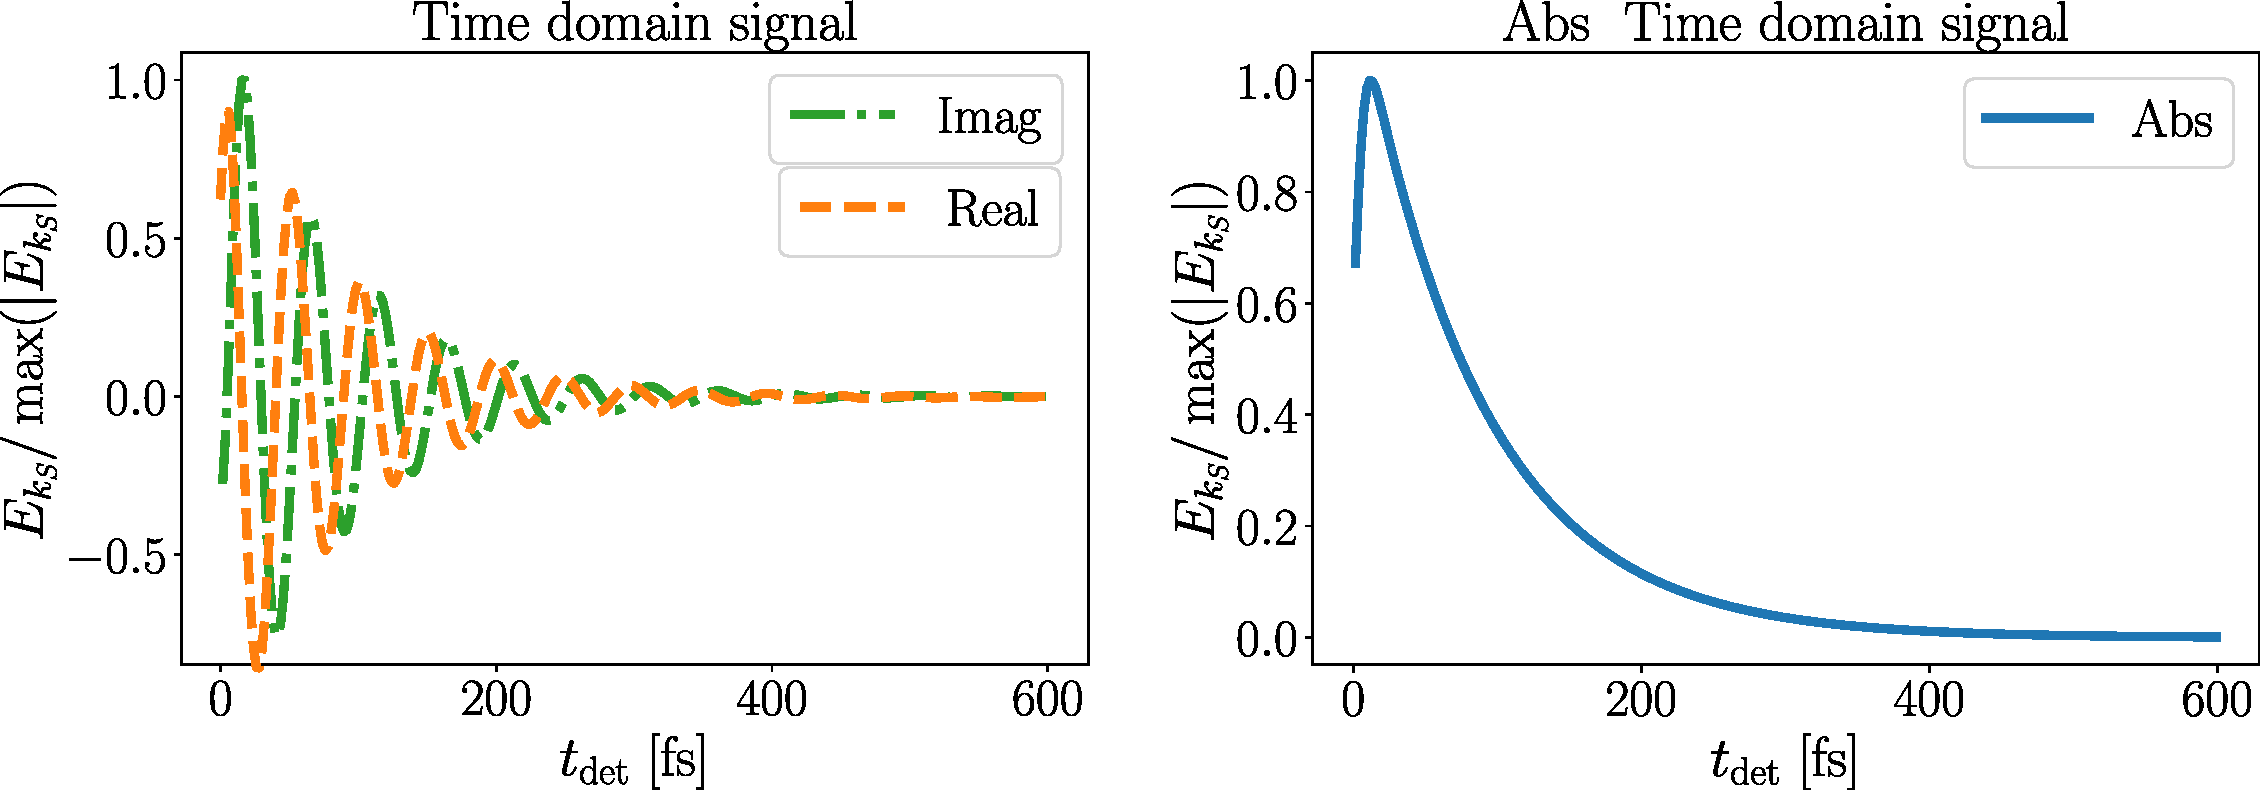
\includegraphics[width=0.85\linewidth]{figures/rslts_tls_hom_rephasing_time_trace.pdf}%
	}{%
		\fbox{\parbox{0.85\linewidth}{\centering\vspace{2mm}
				Placeholder: 1D rephasing time trace for a qubit.\\
				Put the file at \texttt{latex/figures/tls\_rephasing\_time\_trace.pdf}.\vspace{2mm}}}%
	}
	\caption{Time-domain three-pulse photon-echo (rephasing) signal of a two-level system computed from the RWA equations of motion, \autoref{eq:model_tls_eom_rhoeg}--\autoref{eq:model_tls_eom_rhogg}, with the paper parameters ($\tau=300\,\mathrm{fs}$, $T=1000\,\mathrm{fs}$, $\gamma^{-1}=300\,\mathrm{fs}$, $T_2^{*}=100\,\mathrm{fs}$, $\tau_{\mathrm{pulse}}=15\,\mathrm{fs}$, $\omega_{eg}=16000\,\mathrm{cm}^{-1}$, and inhomogeneous FWHM $\Delta_{\mathrm{inh}}=200\,\mathrm{cm}^{-1}$) at resonance $\omega_{L}=\omega_{eg}$. This reproduces the reference result of \cite{mancaletal2006twodimensionalopticalthreepulse}.}
	\label{fig:model_tls_hom_rephasing_time_trace}
\end{figure}

The homogeneous case is shown in~\autoref{fig:model_tls_2d_spectra_homogeneous}.
\begin{figure}[htbp]
	\centering
	\IfFileExists{figures/tls_2d_spectra_homogeneous.pdf}{%
		\includegraphics[width=0.95\linewidth]{figures/tls_2d_spectra_homogeneous.pdf}%
	}{%
		\fbox{\parbox{0.95\linewidth}{\centering\vspace{2mm}
				Placeholder: qubit 2D spectra vs waiting time $T$ (homogeneous broadening).\\
				Put the file at \texttt{latex/figures/tls\_2d\_spectra\_homogeneous.pdf}.\vspace{2mm}}}%
	}
	\caption{Sequence of rephasing/nonrephasing (or absorptive) 2D spectra of a homogeneously broadened qubit for increasing waiting time $T$. Solid/dashed contours indicate positive/negative contributions as in standard 2D-FTS conventions. (This placeholder should be replaced by the corresponding figure set.)}
	\label{fig:model_tls_2d_spectra_homogeneous}
\end{figure}

The inhomogeneous case is shown in~\autoref{fig:model_tls_2d_spectra_inhomogeneous}.
\begin{figure}[htbp]
	\centering
	\IfFileExists{figures/tls_2d_spectra_inhomogeneous.pdf}{%
		\includegraphics[width=0.95\linewidth]{figures/tls_2d_spectra_inhomogeneous.pdf}%
	}{%
		\fbox{\parbox{0.95\linewidth}{\centering\vspace{2mm}
				Placeholder: qubit 2D spectra vs waiting time $T$ (inhomogeneous broadening).\\
				Put the file at \texttt{latex/figures/tls\_2d\_spectra\_inhomogeneous.pdf}.\vspace{2mm}}}%
	}
	\caption{Sequence of 2D spectra of an inhomogeneously broadened qubit ensemble for increasing waiting time $T$. Compared to \autoref{fig:model_tls_2d_spectra_homogeneous}, static disorder produces an elongated diagonal feature, while homogeneous dynamics govern the antidiagonal width. (This placeholder should be replaced by the corresponding figure set.)}
	\label{fig:model_tls_2d_spectra_inhomogeneous}
\end{figure}

\subsection{From TLS to Multilevel Manifolds}
\label{sec:model_tls_to_multilevel}

The two-level system above is a pedagogical reference model. The actual simulations in this thesis are formulated in a multilevel excitation-manifold picture, where the Hilbert space is organized into
\begin{itemize}
\item a ground manifold $\ket{g}$,
\item a single-excitation manifold $\{\ket{n}\}$, and
\item a double-excitation manifold $\{\ket{f}\}$.
\end{itemize}
Within this structure, third-order signals naturally separate into three physical classes during the waiting interval $T$: ground-state bleach (GSB), stimulated emission (SE), and excited-state absorption (ESA).
GSB and SE are already present in the strict TLS limit, whereas ESA requires the additional $\ket{f}$ manifold and corresponds to transitions $n\rightarrow f$ after population has been prepared in the single-excitation manifold.
Because the $g\rightarrow n$ and $n\rightarrow f$ transition frequencies generally differ, ESA often appears at shifted detection frequencies and can carry sign opposite to GSB/SE in differential spectra.

To make the pathway language used later in this chapter explicit, \autoref{tab:model_pathway_classification} summarizes the generic mapping between pathway families, phase character, and physical classes.
\begin{table}[htbp]
\centering
\caption{Generic classification of third-order pathways in the multilevel model. In practice, each pathway family can contain GSB, SE, or ESA contributions depending on the intermediate state occupied during $T$ and on the available level structure.}
\label{tab:model_pathway_classification}
\begin{tabular}{c c l l}
\hline\hline
Pathway & Rephasing/ & State during $T$ & Physical class \\
family & nonrephasing & (examples) & (examples) \\
\hline
$R_1$ & nonrephasing & $\ket{g}\!\bra{g}$ or $\ket{n}\!\bra{n}$ & GSB, SE, or ESA \\
$R_2$ & rephasing & $\ket{g}\!\bra{g}$ or $\ket{n}\!\bra{n}$ & GSB, SE, or ESA \\
$R_3$ & rephasing & $\ket{g}\!\bra{g}$ or $\ket{n}\!\bra{n}$ & GSB, SE, or ESA \\
$R_4$ & nonrephasing & $\ket{g}\!\bra{g}$ or $\ket{n}\!\bra{n}$ & GSB, SE, or ESA \\
\hline\hline
\end{tabular}
\end{table}


%-------------------------------------------------------------------------------
% 2. Dimer (two coupled sites)
%-------------------------------------------------------------------------------

\section{Dimer (Two Coupled Sites)}
\label{sec:model_dimer}


As the next step, a dimer is considered: two optically active sites with a possible coherent coupling constant $J$. This is the minimal model that can produce cross peaks and coupling-induced spectral structure in 2D spectra, and it is a natural bridge to larger ensembles.

\subsection{Manifolds and Basis States}


The standard excitation-manifold basis is used. The ground state is $\ket{g}$. The singly excited manifold is spanned by two localized excitations $\ket{1}$ and $\ket{2}$ (``site basis''), and the doubly excited state is $\ket{f}\equiv\ket{12}$.
This matches the \, $\ket{g},\ket{n},\ket{f}$ scheme discussed in~\autoref{chapter:spctr_spectroscopy} with $n\in\{1,2\}$.

\subsection{Hamiltonian with Coupling \texorpdfstring{$J$}{J}}


In the single-excitation manifold, the Hamiltonian is taken as
\begin{equation*}
	\hat{H}_{0}^{(\mathrm{dimer})}
	= \varepsilon_1\,\ket{1}\!\bra{1} + \varepsilon_2\,\ket{2}\!\bra{2}
	+ J\,\big(\ket{1}\!\bra{2}+\ket{2}\!\bra{1}\big)
	\; +\; (\varepsilon_1+\varepsilon_2)\,\ket{f}\!\bra{f}.
\end{equation*}
Setting $J=0$ recovers two uncoupled transitions. Finite $J$ produces excitonic eigenstates and characteristic peak splittings/cross peaks in 2D spectra.

\subsection{Exciton Basis (Useful Limiting Picture)}


For interpretation of spectra it is often useful to diagonalize the single-excitation block. Introducing the site-energy difference $\Delta\varepsilon=\varepsilon_1-\varepsilon_2$, the two single-exciton eigenenergies are
\begin{equation*}
	\varepsilon_{\pm} = \tfrac{1}{2}(\varepsilon_1+\varepsilon_2) \pm \sqrt{\big(\tfrac{\Delta\varepsilon}{2}\big)^2 + J^2}.
\end{equation*}
The corresponding eigenstates $\ket{\pm}$ interpolate between localized excitations (for $|J|\ll |\Delta\varepsilon|$) and fully delocalized superpositions (for $|J|\gg |\Delta\varepsilon|$). In the 2D spectrum this coherent mixing is visible already at waiting time $T=0$ through peak splittings and, generically, non-vanishing off-diagonal structure.

\subsection{Dipole Operator}


The dipole operator is written as the sum over allowed one-quantum transitions,
\begin{equation*}
	\hat{\mu}^{(\mathrm{dimer})}
	= \sum_{n=1}^{2} \Big(\mu_{gn}\,\ket{g}\!\bra{n} + \mu_{ng}\,\ket{n}\!\bra{g}\Big)
	+ \sum_{n=1}^{2} \Big(\mu_{nf}\,\ket{n}\!\bra{f} + \mu_{fn}\,\ket{f}\!\bra{n}\Big),
\end{equation*}
with $\mu_{ng}=\mu_{gn}^*$ and $\mu_{fn}=\mu_{nf}^*$. The $\ket{n}\leftrightarrow\ket{f}$ transitions are required to include excited-state absorption pathways in third-order response.

\subsection{Excited-State Absorption in the Dimer}
\label{sec:model_dimer_esa}

Real molecular aggregates rarely behave as strict two-level systems. In the dimer, after optical excitation from $\ket{g}$ into the single-excitation manifold ($\ket{1},\ket{2}$ or equivalently $\ket{\pm}$), additional absorption into the doubly excited state $\ket{f}$ becomes possible. This process is the excited-state absorption (ESA) contribution.

In Liouville-space language, ESA pathways are obtained from the pathways that pass through excited-state population during the waiting interval $T$, followed by a final interaction that creates an $f\leftrightarrow n$ coherence ($n\in\{1,2\}$ or $n\in\{+, -\}$). The emitted field then oscillates near the corresponding transition frequency $\omega_{fn}$. As in the two-level rephasing/nonrephasing decomposition, ESA appears in both rephasing and nonrephasing branches.

At the response-function level, ESA pathways enter with opposite sign to GSB/SE. With the standard pump--probe differential-absorption convention, however, this sign is inverted once more, so ESA is observed as a positive contribution around detection frequencies close to $\omega_{fn}$. A compact schematic form is
\begin{equation*}
	\Delta A_{\mathrm{ESA}}(\omega;T)
	\propto
	+\,\omega\,\sum_{n}
	\bigl|d_{fn}\,d_{ng}\bigr|^2\,
	\Re\,g_{fn}(\omega)\,
	\mathrm{e}^{-k_{ng}T},
\end{equation*}
where $g_{fn}(\omega)$ is the line-shape function for the $n\to f$ transition, $d_{ng}$ and $d_{fn}$ are transition dipole moments, and $k_{ng}$ denotes the effective decay rate of the corresponding excited-state population channel.

This is the key mechanism behind partial cancellation in pump--probe and absorptive 2D spectra: GSB and SE produce negative features near $\omega_{ng}$, while ESA produces positive features near $\omega_{fn}$. If these frequencies and linewidths overlap, nodal lines and reduced net amplitudes can appear even when each individual contribution is substantial.

For waiting-time dynamics, SE and ESA typically decay with the surviving excited-state population, whereas GSB contains both a static bleach component and a refilling component through population return to $\ket{g}$. In the long-time limit, all transient contributions vanish as the system relaxes back to the ground state.


The specific dimer parameter choices and the figures to be shown for the dimer will be specified later.

\subsection{Physical Interpretation in 2D Spectra: Coupling vs. Transfer}
\label{sec:model_dimer_interpretation}


This dimer is the minimal setting in which the 2D spectrum can distinguish qualitatively different ``excitation-transfer'' mechanisms:
\begin{itemize}
	\item \textbf{Coherent coupling (excitonic mixing).} For $J\neq 0$ the optical transitions are between $\ket{g}$ and the exciton states $\ket{\pm}$ (and, if included, between $\ket{\pm}$ and $\ket{f}$). In this case cross peaks can be present already at $T=0$ because the eigenstates are delocalized and the Liouville pathways do not cancel exactly.
	\item \textbf{Incoherent population transfer.} If the sites are only weakly coupled (or even uncoupled) but the environment induces population transfer $\ket{1}\to\ket{2}$ (or both directions), then cross peaks are typically \emph{absent at $T=0$} and \emph{grow with $T$} as population migrates during the waiting time. In this scenario diagonal peak amplitudes decay while the corresponding cross peak rises on the same timescale.
\end{itemize}


This ``$T=0$ cross peak'' versus ``growth with $T$'' distinction is a convenient rule of thumb when interpreting simulated (or measured) spectra.

\subsection{Transfer Model During the Waiting Time}
\label{sec:model_dimer_transfer_model}


To model unidirectional or bidirectional excitation transfer within the single-excitation manifold during the waiting interval $T$, the coherent Hamiltonian evolution may be complemented by Lindblad jump operators of the form
\begin{equation*}
	\hat{L}_{2\leftarrow 1} = \sqrt{k_{2\leftarrow 1}}\,\ket{2}\!\bra{1},
	\qquad
	\hat{L}_{1\leftarrow 2} = \sqrt{k_{1\leftarrow 2}}\,\ket{1}\!\bra{2},
\end{equation*}
in addition to site-local relaxation/dephasing operators (\autoref{chapter:oqs_open_quantum_systems}). In the numerical workflow this affects the evolution superoperator acting between the second and third interactions and therefore controls the waiting-time dependence of diagonal and cross-peak amplitudes.

\subsection{Coherences During \texorpdfstring{$T$}{T} (Oscillatory Peak Dynamics)}
\label{sec:model_dimer_coherences}


If the system supports excited-state coherences during the waiting time (e.g. between $\ket{+}$ and $\ket{-}$), then selected peak amplitudes can acquire oscillatory $T$-dependence at the exciton splitting frequency (with a decay set by the corresponding dephasing rate). In practice, this provides a direct numerical handle to separate ``population transfer'' signatures (monotonic rise/decay) from coherence signatures (beats) in the same model.

%-------------------------------------------------------------------------------
% 3. N-site ensemble with geometry
%-------------------------------------------------------------------------------

\section{Generalization to an \texorpdfstring{$N$}{N}-Site Ensemble with Geometry}
\label{sec:model_ensemble}


Finally, an ensemble of $N$ optically active sites (``atoms'' or chromophores) placed in a prescribed geometry is considered. Motivated by protofilament arrangements in microtubules, the geometry of interest in this thesis is a discretized cylindrical surface \cite{kalraetal2023electronicenergymigration}. The model is formulated in the excitation-manifold basis \,$\ket{g},\{\ket{n}\},\{\ket{f}\}$ already used in~\autoref{chapter:spctr_spectroscopy}.

\subsection{States and Truncation}


The ground state is $\ket{g}$. The single-excitation manifold is spanned by states $\ket{n}$, $n\in\{1,\dots,N\}$, which represent one excitation localized at site $n$ (or, after diagonalization, an excitonic eigenstate). If double excitations are included, states $\ket{f}\equiv\ket{mn}$ with $1\le m<n\le N$ are used, representing two simultaneous excitations.
In this thesis the Hilbert space is restricted to the ground state plus the single-excitation manifold, or (when needed for ESA contributions) to ground + single + double excitations.

\subsection{What 2D Spectra Diagnose in Ensembles}
\label{sec:model_ensemble_interpretation}


In an $N$-site setting, 2D spectra are particularly useful because they separate several effects that are difficult to disentangle in linear absorption:
\begin{itemize}
	\item \textbf{Static disorder (inhomogeneous broadening)} produces elongation along the diagonal in the $(\omega_{\mathrm{coh}},\omega_{\mathrm{det}})$ plane, reflecting a distribution of transition frequencies across realizations.
	\item \textbf{Homogeneous dephasing} controls the antidiagonal width (for fixed disorder), i.e.	he width perpendicular to the diagonal, and therefore provides access to dephasing timescales even in disordered ensembles.
	\item \textbf{Transport and transfer} redistribute amplitude between diagonal and off-diagonal features as a function of $T$. The pattern of emerging cross peaks encodes which states (or spatial regions) become correlated during the waiting time.
\end{itemize}

These qualitative diagnostics motivate the use of 2D-FTS observables as a readout for geometry-dependent excitation migration in the cylindrical architectures studied below.

\subsection{Hamiltonian}


In this basis, a generic Frenkel-exciton-type Hamiltonian reads
\begin{equation*}
	\hat{H}_{0}^{(N)}
	= \sum_{n=1}^{N} \varepsilon_n\,\ket{n}\!\bra{n}
	+ \sum_{m<n}^{N} J_{mn}\,\big(\ket{m}\!\bra{n}+\ket{n}\!\bra{m}\big)
	+ \sum_{m<n}^{N} (\varepsilon_m+\varepsilon_n)\,\ket{mn}\!\bra{mn}
	+ \cdots,
\end{equation*}
where $\varepsilon_n$ are site transition frequencies and $J_{mn}$ are coherent couplings.
The ellipsis indicates additional terms in the double-excitation manifold if one wishes to include interactions beyond an additive two-exciton energy (e.g. exciton--exciton shifts).

\subsection{Geometry and Couplings}


The couplings $J_{mn}$ may be parameterized phenomenologically (e.g. nearest-neighbour) or computed from transition-dipole interactions. In the latter case one uses
\begin{equation*}
	J_{mn} \propto \frac{1}{ \lVert \boldsymbol{r}_{mn} \rVert^{3} }
	\left[
		\boldsymbol{\mu}_m \cdot \boldsymbol{\mu}_n
		- 3\,(\boldsymbol{\mu}_m \cdot \hat{\boldsymbol{r}}_{mn})(\boldsymbol{\mu}_n \cdot \hat{\boldsymbol{r}}_{mn})
		\right],
\end{equation*}
with site positions $\boldsymbol{r}_n$ and displacement $\boldsymbol{r}_{mn}=\boldsymbol{r}_m-\boldsymbol{r}_n$ \cite{griffiths2013introductionelectrodynamics,lehmberg1970radiationatomsystem,masters2014pathsforstersresonance}.


For a cylindrical arrangement, let $N_{\theta}$ be the number of sites per ring and $N_z$ the number of rings (so $N=N_{\theta}N_z$), with sites indexed by an azimuthal index and an axial index. Periodic boundary conditions can be imposed in the azimuthal direction.

\subsection{Dipole Operator}


The dipole operator is the sum over allowed one-quantum transitions between adjacent excitation manifolds,
\begin{equation*}
	\hat{\mu}^{(N)}
	= \sum_{n=1}^{N} \Big(\mu_{gn}\,\ket{g}\!\bra{n} + \mu_{ng}\,\ket{n}\!\bra{g}\Big)
	+ \sum_{m<n}^{N} \sum_{\ell\in\{m,n\}} \Big(\mu_{\ell,mn}\,\ket{\ell}\!\bra{mn} + \mu_{mn,\ell}\,\ket{mn}\!\bra{\ell}\Big),
\end{equation*}
where the second sum is only needed if the double-excitation manifold is included.


This model class captures collective transport pathways and their photon-echo signatures, offering a route to connect microscopic couplings and geometry to observable 2D spectra \cite{kalraetal2023electronicenergymigration}.


\todoidea{Include this:}


\subsubsection{Multilevel Generalization}
\label{sec:model_multilevel_generalization}
Realistic systems typically have many optically accessible excited states, and a central goal of this thesis is to extend the simulation framework from a minimal two-level model to multilevel Hamiltonians. A convenient (and widely used) idealisation that already captures the essential physics of ground-state bleach (GSB), stimulated emission (SE), and excited-state absorption (ESA) is a three-manifold ``band'' picture:
\begin{itemize}
	\item a single ground state $\ket{g}$.
	\item a manifold of singly excited states $\{\ket{n}\}$.
	\item a manifold of higher excited (doubly excited) states $\{\ket{f}\}$.
\end{itemize}
Optically allowed transitions connect $\ket{g}\leftrightarrow\ket{n}$ and $\ket{n}\leftrightarrow\ket{f}$. In third-order spectroscopy the Liouville pathways do not contain populations of the $f$ manifold (they end in coherences such as $\rho_{fn}$), so relaxation out of $f$ typically enters effectively through additional dephasing/broadening of the $n\leftrightarrow f$ coherences.

\medskip

\textbf{Propagators in the secular approximation.}
In the secular approximation, the $\tau_2$ evolution is expressed in terms of Liouville-space propagator elements of the generic form
\begin{equation*}
	U_{nn,mm}(\tau_2),\qquad U_{nm,nm}(\tau_2),\qquad U_{gg,nn}(\tau_2),
\end{equation*}
describing population transfer within the excited manifold ($nn\to mm$), coherence dephasing within the excited manifold ($nm\to nm$), and refilling of the ground state from excited populations ($nn\to gg$). ESA pathways additionally involve propagators for $f$-manifold coherences (e.g. $U_{fn,fm}(\tau_2)$).

\medskip

\textbf{Recipe for constructing multilevel signals.}
Given these propagators, multilevel spectra are obtained by the same ``stitching'' procedure as in the two-level case:
\begin{enumerate}
	\item choose the relevant pulse sequence (and thus the allowed pathway classes and phase matching / phase cycling).
	\item for each pathway, write the product of four dipole matrix elements (e.g. $d_{ng}$, $d_{mg}$, and, for ESA, $d_{fn}$) and three propagators (coherence--population--coherence) appropriate to that pathway.
	\item Fourier transform over the detection time to obtain contributions as functions of $\omega_{\mathrm{det}}$ (and, for 2D spectra, also over the coherence time to obtain $\omega_{\mathrm{coh}}$).
	\item sum over all intermediate state indices $n,m,f,\dots$.
\end{enumerate}


This multilevel bookkeeping is exactly what becomes necessary once the system Hamiltonian contains multiple excited eigenstates (or excitonic bands) and the open-system Liouvillian generates non-trivial transfer and dephasing within these manifolds. The explicit multilevel formulation will therefore serve as the bridge from the pedagogical two-level picture to the full numerical simulations targeted in the later thesis chapters.

\medskip

\textbf{General dissipative channels (preview).}
For later use it is helpful to note that a multilevel relaxation model can be written compactly in Lindblad form by introducing one jump operator per allowed transition $\ket{n}\to\ket{m}$,
\begin{equation*}
	\hat{L}_{mn} = \sqrt{k_{mn}}\,\ket{m}\bra{n},
\end{equation*}
and, if needed, pure-dephasing operators for each level,
\begin{equation*}
	\hat{L}_{n}^{(\varphi)} = \sqrt{\gamma_{\varphi,n}}\,\ket{n}\bra{n}.
\end{equation*}
These ingredients define the Liouvillian whose propagator elements $U_{ab,cd}(t)$ enter directly in the pathway products described above.

\todoimp{at the correct point implement this:}
In a chosen basis $\{\ket{n}\}$ of the system Hilbert space \autoref{eq:spctr_P_def_spectroscopy} becomes 
\begin{equation*}
	\boldsymbol{P}(t)=\sum_{n,m}
	\boldsymbol{\mu}_{nm}\,\rho_{S,mn}(t),
	\qquad
	\boldsymbol{\mu}_{nm}=\bra{n}\hat{\boldsymbol{\mu}}\ket{m}.
\end{equation*}
Oscillating polarisation is generated by optical coherences, i.e.\ off-diagonal elements of the density matrix. If the relevant electronic states carry no permanent dipoles in the chosen eigenbasis, i.e.\ $\boldsymbol{\mu}_{nn}=\boldsymbol{0}$, then populations do not contribute.

\todoidea{implement this somewhere: Scanning the waiting time $t_{\mathrm{wait}}$ probes population dynamics and spectral diffusion during the population interval between the second and third interactions~\cite{cho2009twodimensionalopticalspectroscopy, mukamel1995principlesnonlinearoptical}.

}
